\documentclass[border=14pt]{standalone}
\usepackage{tikz}
\usetikzlibrary{arrows.meta,positioning,shapes.geometric,shapes.misc,calc}
% --- dark theme (matches the tool's slate-900 panels) ---
\definecolor{bg}{HTML}{0F172A}       % background
\definecolor{boxfill}{HTML}{1E293B}  % operators
\definecolor{methfill}{HTML}{334155} % nodes / methods
\definecolor{stroke}{HTML}{64748B}
\definecolor{txt}{HTML}{E2E8F0}
\definecolor{arrowc}{HTML}{94A3B8}
\pagecolor{bg}
\begin{document}
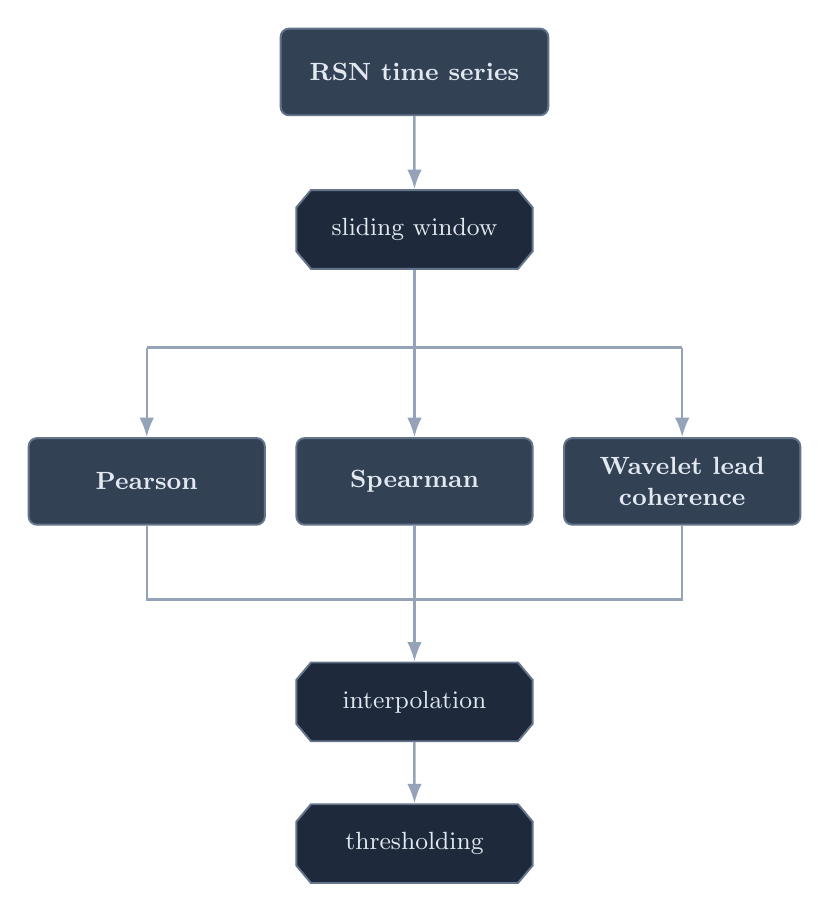
\begin{tikzpicture}[
  >=Latex,
  every node/.style={text=txt},
  proc/.style={rounded corners=3pt, draw=stroke, line width=0.7pt, fill=methfill,
     align=center, inner sep=5pt, minimum height=11mm, minimum width=34mm,
     font=\bfseries\small},
  meth/.style={proc, minimum width=30mm},
  op/.style={chamfered rectangle, chamfered rectangle angle=40,
     draw=stroke, line width=0.7pt, fill=boxfill,
     align=center, inner sep=3pt, minimum height=10mm, minimum width=30mm, font=\small},
  arr/.style={->, line width=0.9pt, draw=arrowc},
  bus/.style={line width=0.9pt, draw=arrowc},
]
% --- rows (top -> bottom) ---
\def\ycol{2.6}
\def\ysw{0.6}
\def\ybus{-0.9}
\def\ymeth{-2.6}
\def\ymerge{-4.1}
\def\yint{-5.4}
\def\ythr{-7.2}
\def\xl{-3.4} \def\xc{0} \def\xr{3.4}
% top chain
\node[proc] (rsn) at (\xc,\ycol) {RSN time series};
\node[op]   (sw)  at (\xc,\ysw)  {sliding window};
% methods row
\node[meth] (pear)  at (\xl,\ymeth) {Pearson};
\node[meth] (spear) at (\xc,\ymeth) {Spearman};
\node[meth] (wav)   at (\xr,\ymeth) {Wavelet lead\\coherence};
% processing
\node[op] (int) at (\xc,\yint) {interpolation};
\node[op] (thr) at (\xc,\ythr) {thresholding};
% --- arrows ---
\draw[arr] (rsn) -- (sw);
% branch sliding window -> methods via horizontal bus
\coordinate (bC) at (\xc,\ybus);
\draw[bus] (sw.south) -- (bC);
\draw[bus] (\xl,\ybus) -- (\xr,\ybus);
\draw[arr] (\xl,\ybus) -- (pear.north);
\draw[arr] (\xc,\ybus) -- (spear.north);
\draw[arr] (\xr,\ybus) -- (wav.north);
% merge methods -> interpolation via horizontal bus
\draw[bus] (pear.south)  -- (\xl,\ymerge)  -- (\xc,\ymerge);
\draw[bus] (wav.south)   -- (\xr,\ymerge)  -- (\xc,\ymerge);
\draw[bus] (spear.south) -- (\xc,\ymerge);
\draw[arr] (\xc,\ymerge) -- (int.north);
% chain
\draw[arr] (int) -- (thr);
\end{tikzpicture}
\end{document}
